
% Diagram (B) - Multiple ellipses reflected into the 4th quadrant with arrows
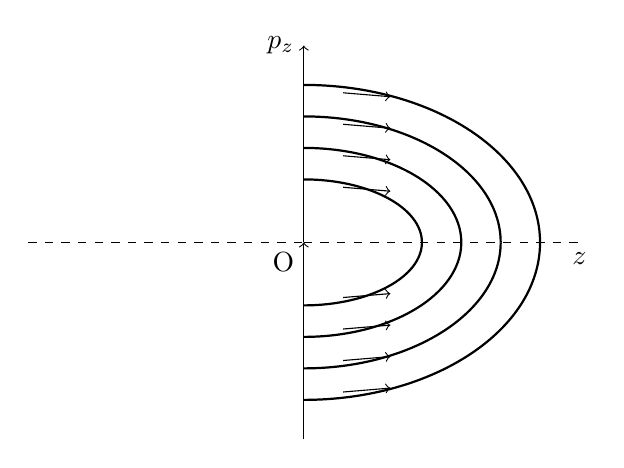
\begin{tikzpicture}
    % Axes
    \draw[->] (0,0) -- (0,2.5) node[left] {$p_z$};
    \draw[->] (0,-2.5) -- (0,0);
    \draw[dashed] (0,0) -- (3.5,0) node[below] {$z$};
    \draw[dashed] (-3.5,0) -- (0,0);
    \node at (0,0) [below left] {O};
    
    % Multiple ellipses (upper parts)
    \draw[thick] (0,2) arc[start angle=90,end angle=0,x radius=3,y radius=2];
    \draw[thick] (0,1.6) arc[start angle=90,end angle=0,x radius=2.5,y radius=1.6];
    \draw[thick] (0,1.2) arc[start angle=90,end angle=0,x radius=2,y radius=1.2];
    \draw[thick] (0,0.8) arc[start angle=90,end angle=0,x radius=1.5,y radius=0.8];
    
    % Reflections (lower parts in the 4th quadrant)
    \draw[thick] (0,-2) arc[start angle=270,end angle=360,x radius=3,y radius=2];
    \draw[thick] (0,-1.6) arc[start angle=270,end angle=360,x radius=2.5,y radius=1.6];
    \draw[thick] (0,-1.2) arc[start angle=270,end angle=360,x radius=2,y radius=1.2];
    \draw[thick] (0,-0.8) arc[start angle=270,end angle=360,x radius=1.5,y radius=0.8];
    
    % Arrows on curves (upper quadrant)
    \draw[->] (0.5,1.9) -- (1.1,1.85);
    \draw[->] (0.5,1.5) -- (1.1,1.45);
    \draw[->] (0.5,1.1) -- (1.1,1.05);
    \draw[->] (0.5,0.7) -- (1.1,0.65);

    % Arrows on curves (lower quadrant)
    \draw[->] (0.5,-1.9) -- (1.1,-1.85);
    \draw[->] (0.5,-1.5) -- (1.1,-1.45);
    \draw[->] (0.5,-1.1) -- (1.1,-1.05);
    \draw[->] (0.5,-0.7) -- (1.1,-0.65);
\end{tikzpicture}


